
\subsection{Operational scenarios}\label{sec:opscenarios}
To study the different aspects of our predictions for the operation of the ITk strip system throughout its lifetime, we performed the calculation of the system parameters over the expected 14 years of operation in monthly steps as outlined in section~\ref{sec:running}. Time-dependent inputs to the calculations were given from the expected performance of the LHC (Fig.~\ref{fig:lhc_profile}) and different profiles for the cooling temperature. We studied flat cooling temperature scenarios at different temperatures starting at $-35^\circ$C, the lowest evaporation temperature achievable with the ITk evaporative CO$_2$ cooling system, and a `ramp' scenario in which the cooling temperature starts at 0$^\circ$C and gradually is lowered down to $-35^\circ$C over the course of 10 years (Fig.~\ref{fig:coolant_ramp}).

\begin{figure}[ht]
\centering
\subfloat[] {\label{fig:lhc_profile}  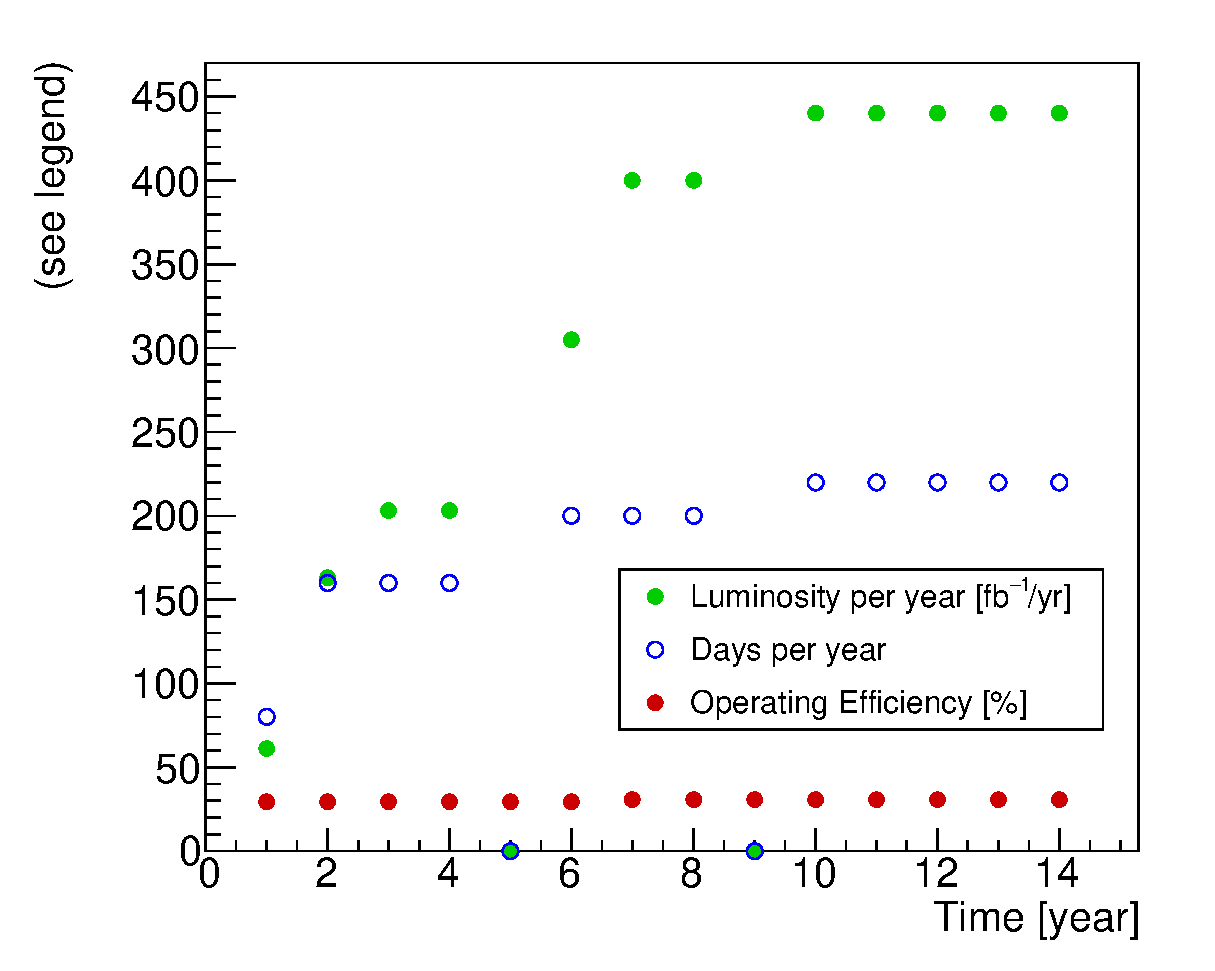
\includegraphics[width=0.45\linewidth]{figures/YearlyRunProfile.eps}}\quad\quad
\subfloat[] {\label{fig:coolant_ramp} 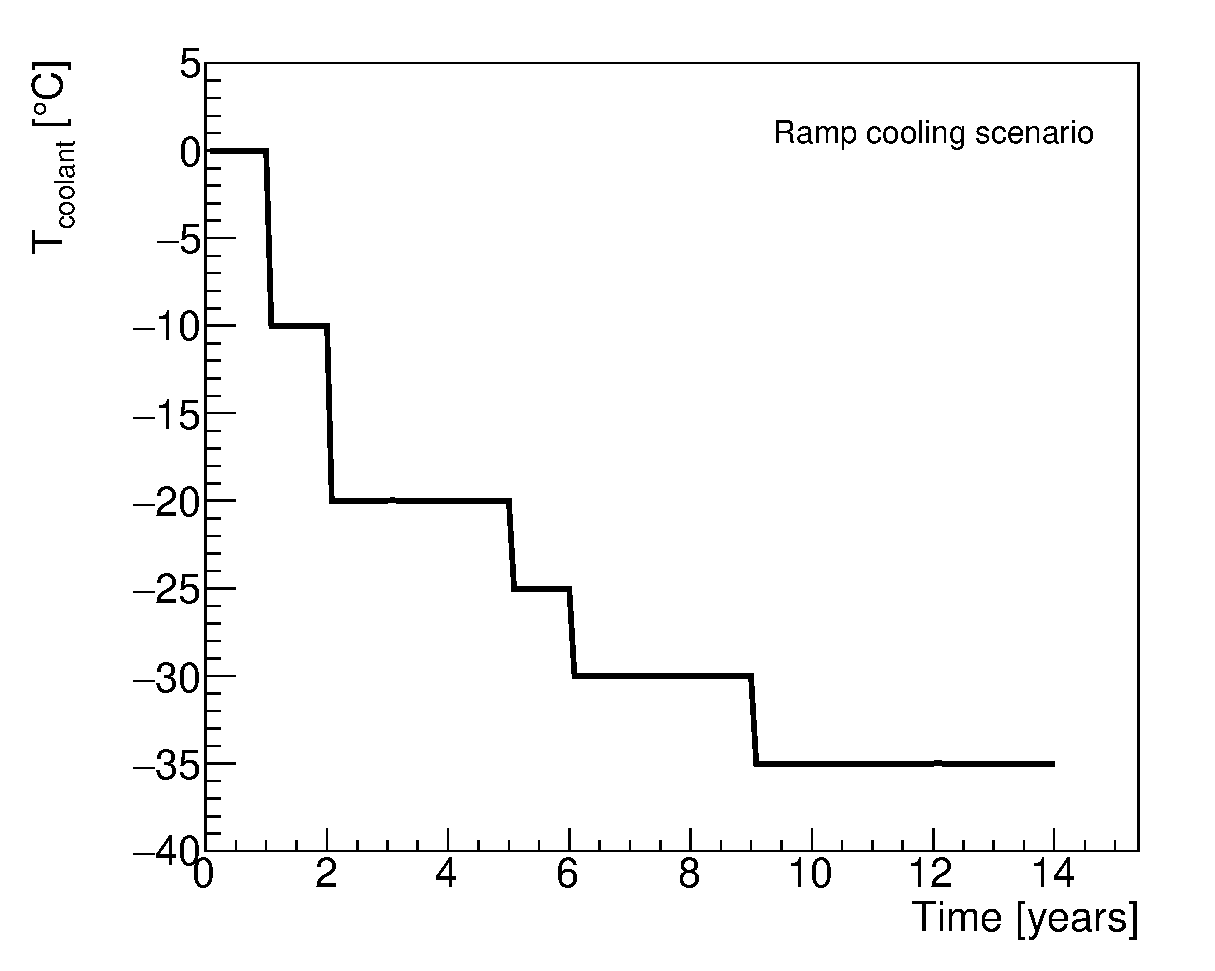
\includegraphics[width=0.45\linewidth]{figures/CoolantTemperature_RampScenario.eps}}
\caption{(a) Expected LHC performance and (b) `cooling ramp' scenario for the coolant temperature. Year-long shutdowns of the LHC are anticipated in years 5 and 9.}
\label{fig:opscenarios}
\end{figure}

\subsection{Safety factors}
\label{sec:safety_factors}
To ensure the robustness of the system design against errors in the assumptions used in the model, we also evaluate the model using a set of input parameters with some key inputs degraded. The set of safety factors used is given in Table~\ref{tab:safetyfactors}. Each safety factor has been estimated individually based on experience, the complexity of the system aspect described by the parameter, and from available data or the absence of such data. Note that the model can be evaluated with all the safety factors listed in Table~\ref{tab:safetyfactors} used together, a situation which is unlikely to occur in the real system, to provide a worst-case estimate for the performance of the ITk strip system. The individual effects of the different safety factors are demonstrated in figure~\ref{fig:safety_factors}.

\let\arraystretcha\arraystretch %% improve the table spacing
\renewcommand\arraystretch{1.2} %% improve the table spacing
\begin{table}[htb]
\caption{Safety factors.}
\label{tab:safetyfactors}
\centering
\adjustbox{max width=\textwidth}{ %% just before tabular
\begin{tabular}{lcl}
\toprule
Safety factor on & Value & Reason \\
\midrule
\multirow{2}{*}{Fluence}  & \multirow{2}{*}{50\%} & Accuracy of fluence calculations and uncertainties\\
                          &                       & in material distributions\\
Thermal impedance & 10\% barrel, 20\% endcap & Local support build tolerances, thermal network assumptions\\
Digital current & 20\% & Final chip performance and parametrization of TID effect\\
Analog current & 5\% & Final chip performance\\
Tape electrical impedance & 10\% & Electrical tape manufacturing tolerances\\
Bias voltage & 700~V & Increased bias voltage from nominal 500~V to maintain S/N\\
TID parametrization & Nominal/Pessimistic & Different data sets for fit of TID bump\\
\bottomrule
\end{tabular}
} %% adjustbox after tabular
\end{table}
\let\arraystretch\arraystretcha %% reset the table spacing

\begin{figure}[ht]
\centering
\subfloat[] {\label{fig:safety_factors_a} 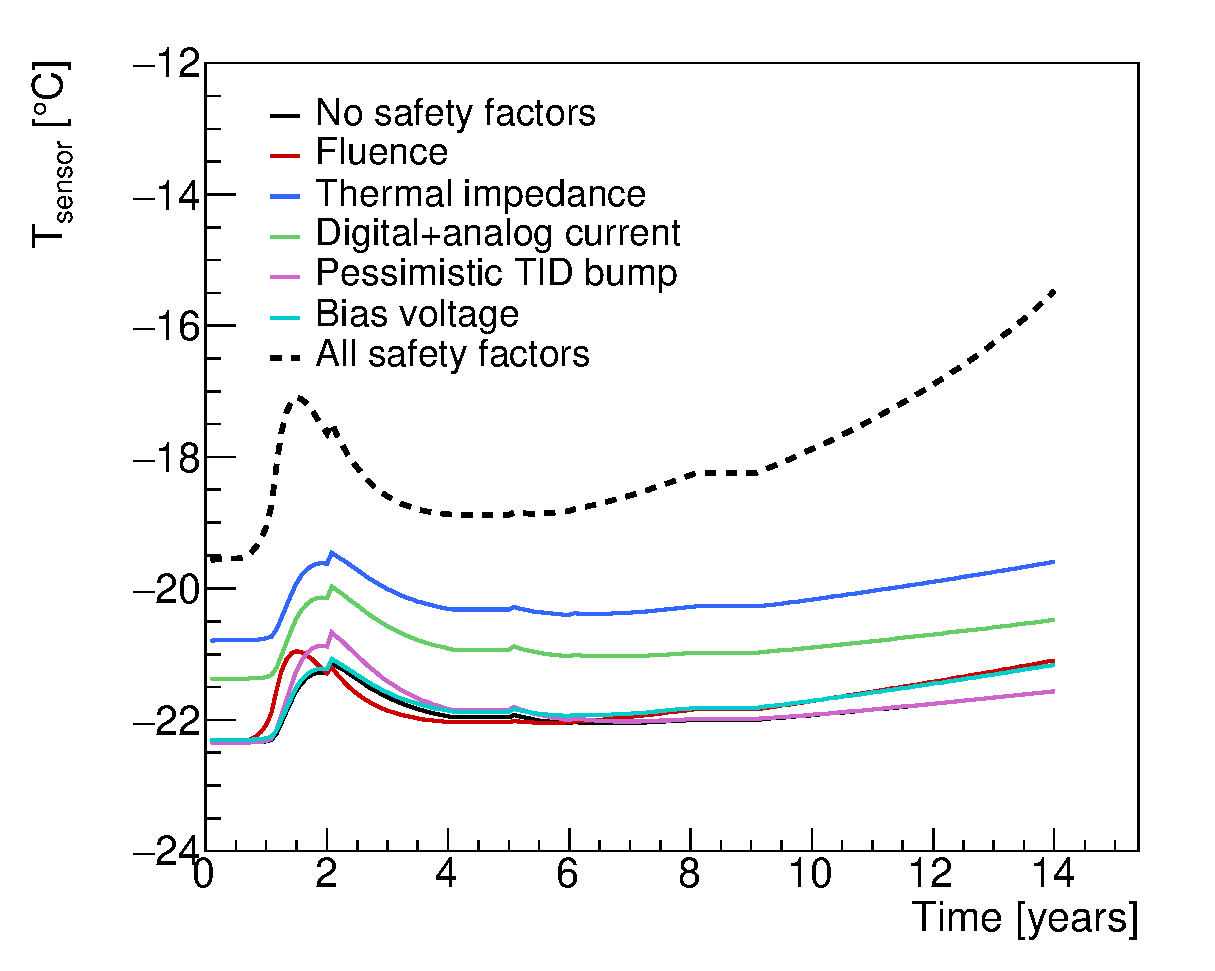
\includegraphics[width=0.45\linewidth]{figures/CompareSafetyFactors_SensorTemperature_R3.eps}}\quad\quad
\subfloat[] {\label{fig:safety_factors_b} 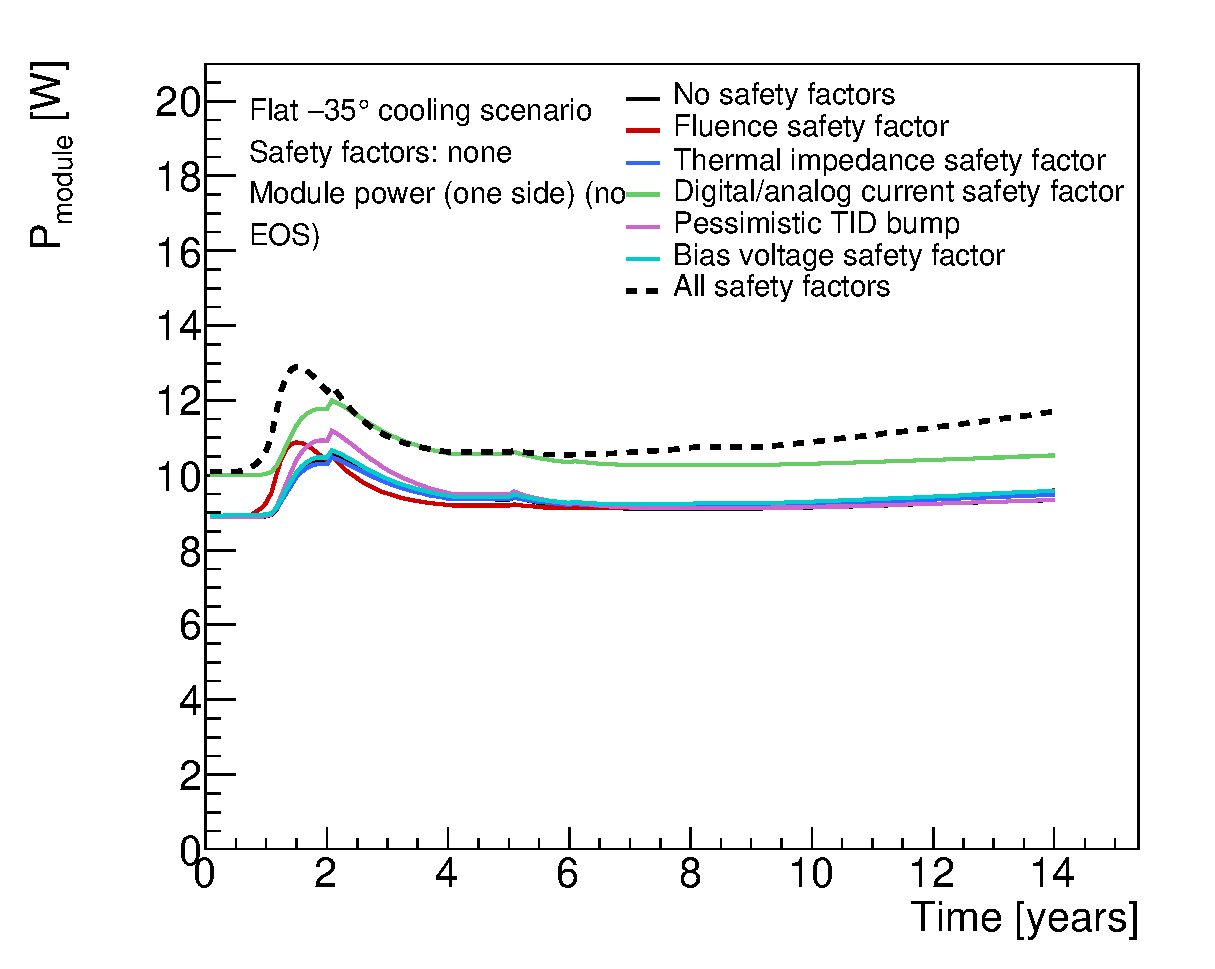
\includegraphics[width=0.45\linewidth]{figures/CompareSafetyFactors_ModulePower_R3.eps}}
\caption{Comparing the impact of different safety factors on (a) the sensor temperature and
(b) the module power for the R3 endcap module. The dotted line depicts the effect of all safety
factors applied at once.}
\label{fig:safety_factors}
\end{figure}

\subsection{Results}
The thermo-electrical model provides a large range of predictions for the operation of the strip system. A detailed discussion of all results would only be of interest to ITk strip system experts and is beyond the scope of this article. Instead we will present here a subset of results to demonstrate the capabilities and use of the thermo-electrical model for the design of the detector system.

\subsubsection{Module properties}

Example output plots of module properties from the thermo-electrical model are shown in Figures~\ref{fig:moduleflatperformance} and~\ref{fig:modulerampperformance}. The different radiation-dependent effects occur on different times scales. The maximum in the digital chip power due to the TID effect occurs relatively early (in year 1 to 4), although the bump has a long tail, particularly in the outer layers of the barrel. The sensor leakage power, on the other hand, grows towards the end of the lifetime of the ITk. If the leakage current continued to increase in the case of further irradiation, or if the cooling termperature were higher, this growth would ultimately lead to thermal runaway. Due to the radial dependence of the radiation environment, the radiation-induced effects are most pronounced in the innermost layers.

\begin{figure}[ht]
\centering
\subfloat[] {\label{fig:moduleflatperformance_a} 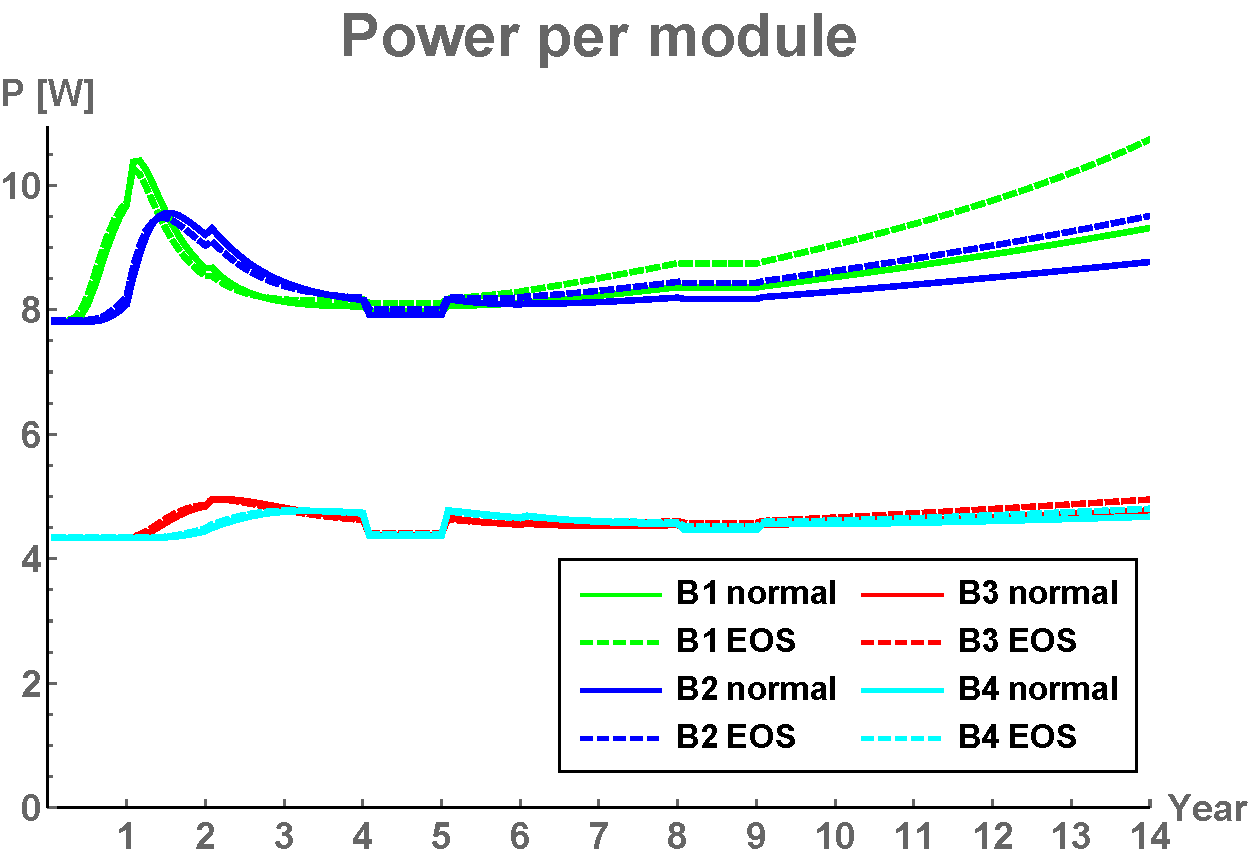
\includegraphics[width=0.4\linewidth]{figures/powerpermodule.pdf}}\quad\quad
\subfloat[] {\label{fig:moduleflatperformance_b} 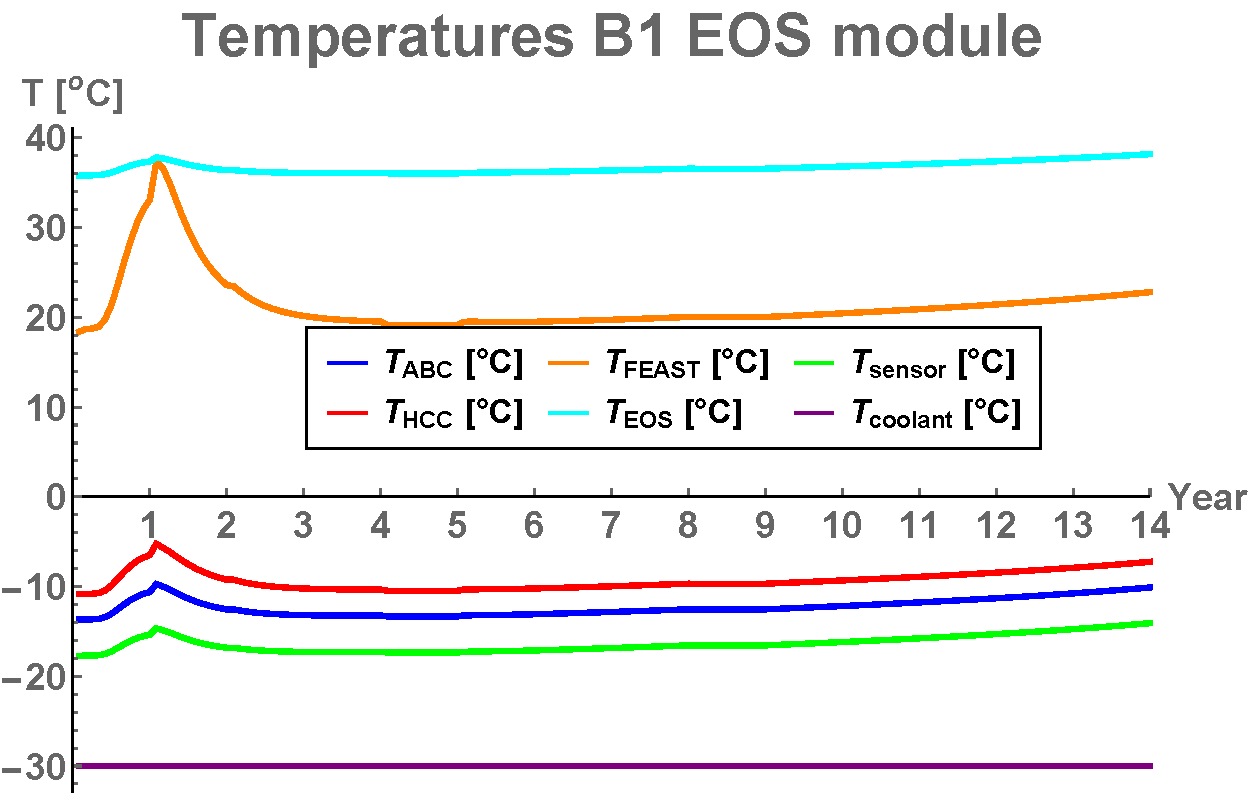
\includegraphics[width=0.4\linewidth]{figures/Teosmodule.pdf}}
\caption{Examples of barrel module performance predictions for a flat cooling scenario ($-30^\circ$) including safety factors. (a) Power per module. (b) Temperatures for different nodes of an end-of-stave barrel module in the innermost barrel.}
\label{fig:moduleflatperformance}
\end{figure}

\begin{figure}[ht]
\centering
\subfloat[] {\label{fig:modulerampperformance_a} 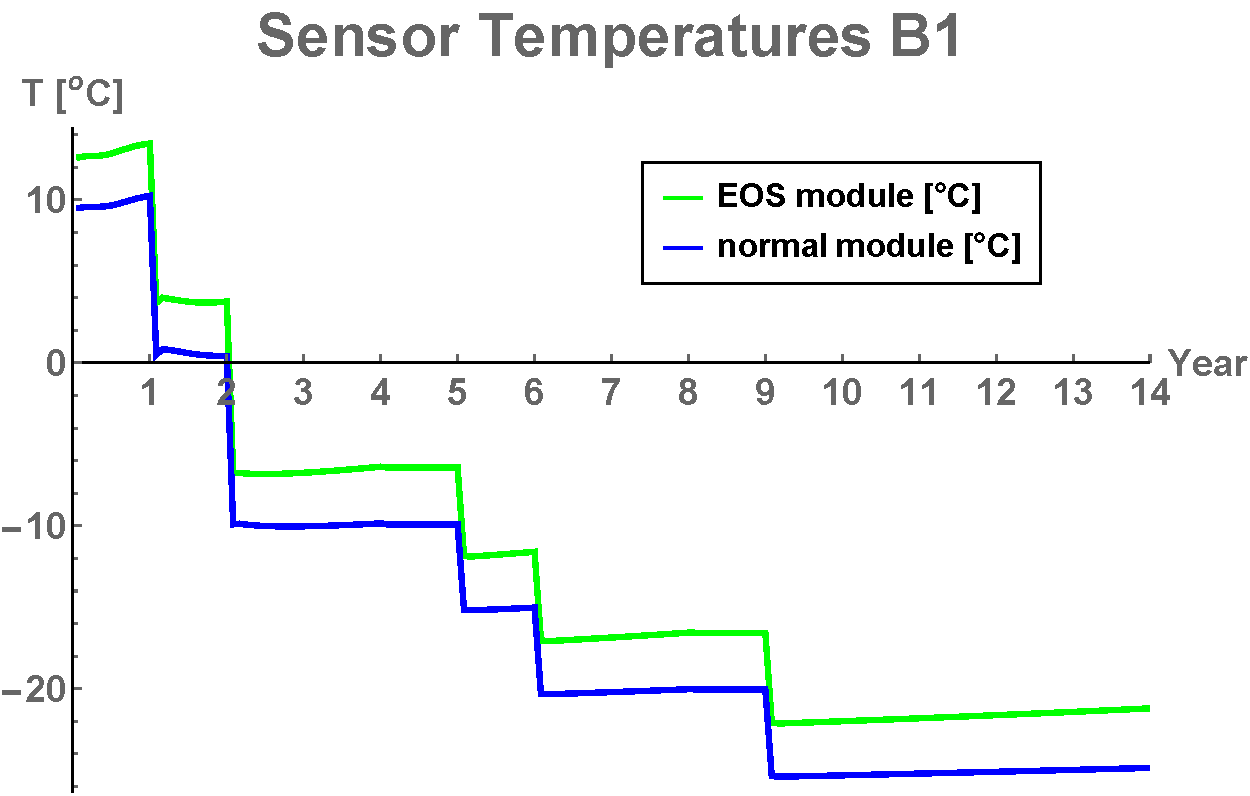
\includegraphics[width=0.4\linewidth]{figures/Tmodule.pdf}}\quad\quad
\subfloat[] {\label{fig:modulerampperformance_b} 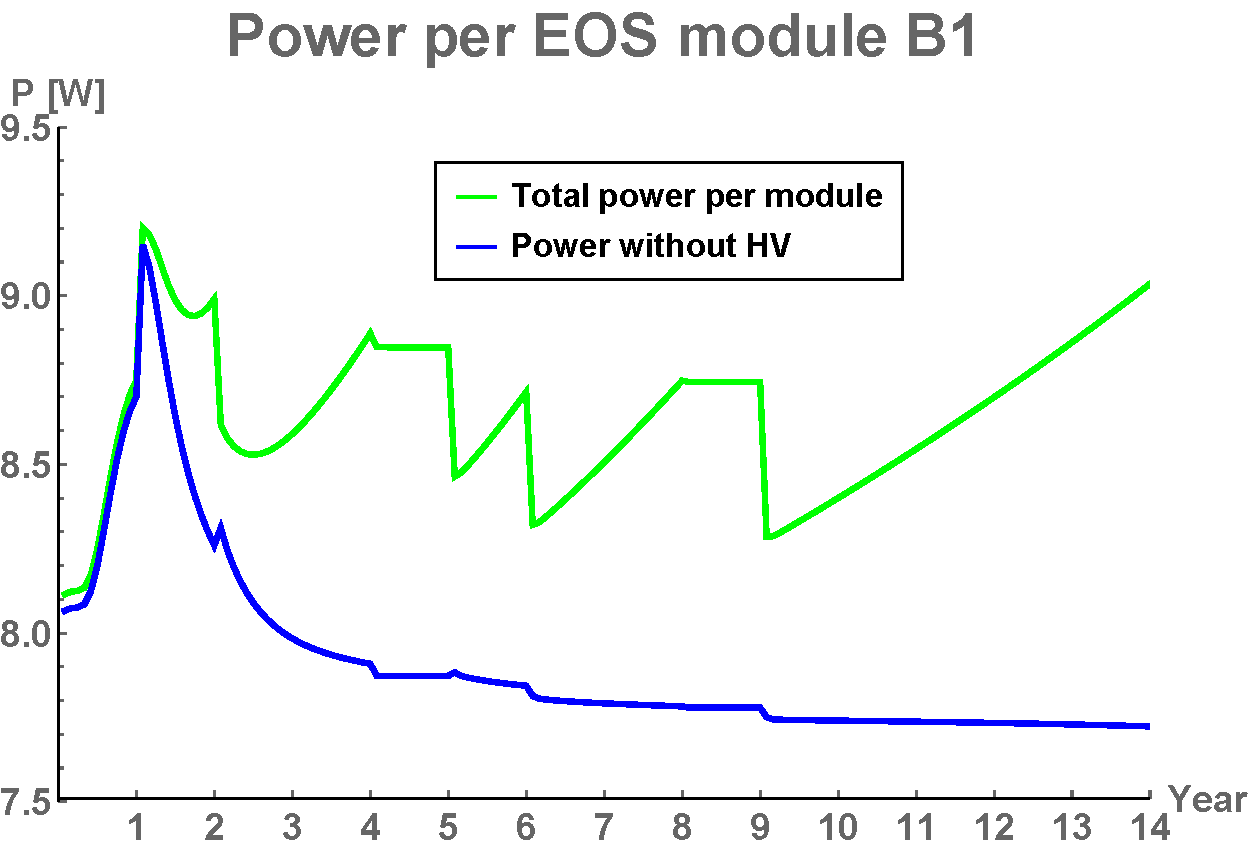
\includegraphics[width=0.4\linewidth]{figures/Peosmodule.pdf}}
\caption{Examples of barrel module performance predictions for the ramp cooling scenario including safety factors. (a) Sensor temperature in the innermost barrel modules. (b) Power in an end-of-stave barrel module in the innermost layer.}
\label{fig:modulerampperformance}
\end{figure}

\subsubsection{System properties}
One of the key concerns for the design of the strip system is thermal stability of the system. If the cooling temperature is too high to limit the leakage power from the radiation-damaged sensors to a level where the heat can still be removed, the system is unstable (it goes into `thermal runaway').
% In this case, there is no solution to the set of equations in the thermo-electrical model anymore, and the numerical search for a solution fails.
% In the barrel strip system, this occurs in the final year of operation at a cooling temperature of $-15^\circ$C under nominal conditions, and at $-25^\circ$C (in year 13) with safety factors applied.
In the endcap strip system, this occurs at a cooling temperature of $-15^\circ$C under nominal conditions; in this scenario, thermal runaway would be reached in the 12$^\text{th}$ year of operation. With safety factors applied, thermal runaway is reached at a cooling temperature of $-25^\circ$C (in year 11).
In the barrel system, where the radiation environment is slightly less intense, the conditions for thermal runaway occur two years later compared to the endcaps.
As the design cooling temperature of the ITk cooling system is $-35^\circ$C, we have confidence that the ITk strip system has sufficient margin for thermal stability.

Beyond the issue of stability, the thermo-electrical model delivers predictions for the development of current and power requirements for the overall system. Some of the predictions are shown in figure~\ref{fig:systemperformance}. Again, the different timescales of the various radiation-induced effects are visible; ignoring this time dependence could lead to overspecification of some system aspects like the total cooling power.

\begin{figure}[ht]
\centering
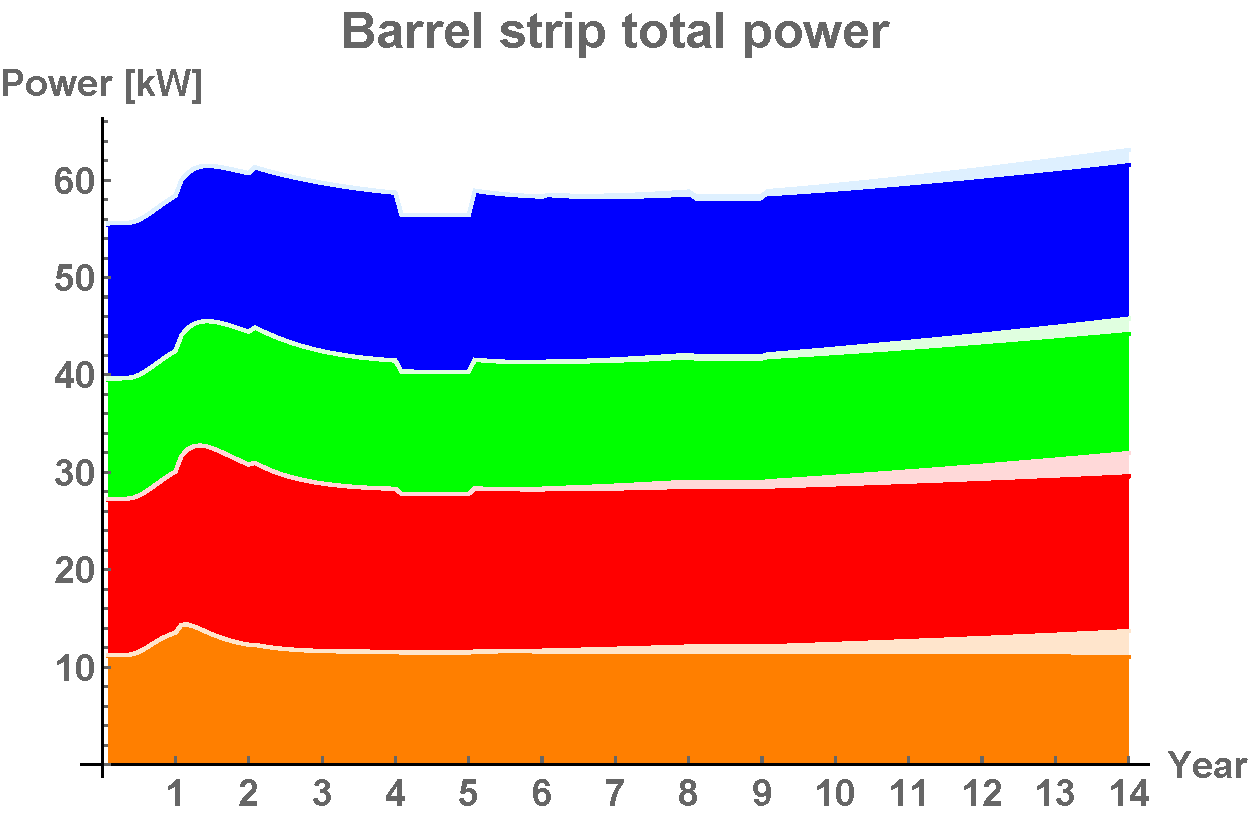
\includegraphics[width=0.4\linewidth]{figures/Totalbarrelpower-30.pdf}
\caption{Examples for system performance predictions. Barrel total power requirements for flat $-30^\circ$ cooling including safety factors (left): The plot shows the stacked power requirements for the four barrels (orange: innermost barrel, blue: outermost barrel). Full colour indicates power from the front-end electronics, greyed parts are contributions from HV power for the four barrels.}
\label{fig:systemperformance}
\end{figure}

These predictions are now used throughout the strip project to consistently size the power supply and cooling systems. Including safety factors in the predictions gives us some confidence that the designs are robust; by using commonly agreed safety factors, we ensure a consistent use of safety factors throughout the project and prevent safety factor creep.

Because of the different timescales for the peak power due to the TID effect and the radiation-induced sensor leakage, there is room to optimize the cooling temperature profile for minimal power. The thermo-electrical model is a powerful tool to plan such an optimized cooling profile. In fact, the cooling `ramp' scenario introduced in Section~\ref{sec:opscenarios} is the result of such an optimization (Fig.~\ref{fig:rampoptimization}).

\begin{figure}[ht]
\centering
\subfloat[] {\label{fig:rampoptimization_a} 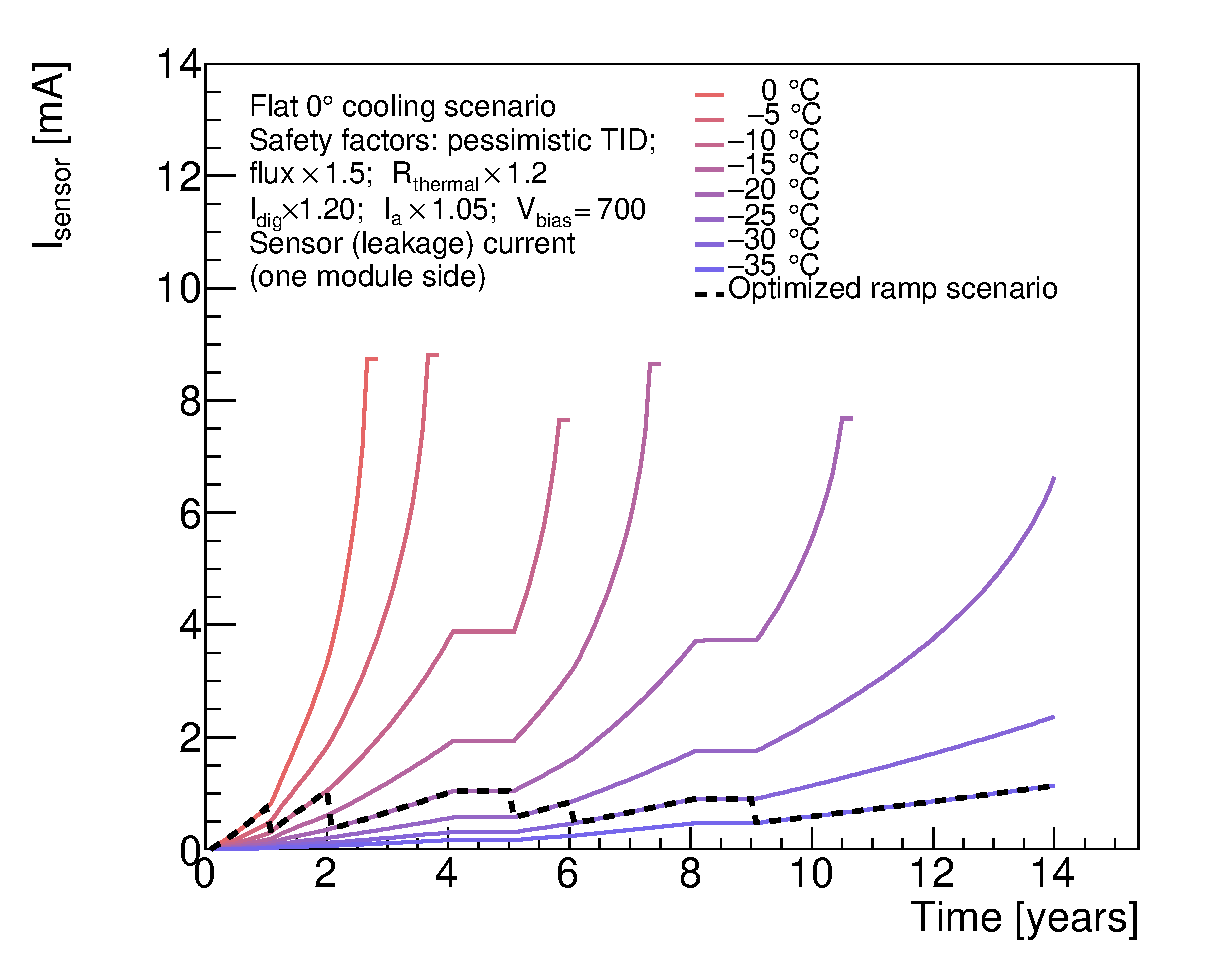
\includegraphics[width=0.45\linewidth]{figures/SensorCurrent_R3_newramp.eps}}\quad\quad
\subfloat[] {\label{fig:rampoptimization_b} 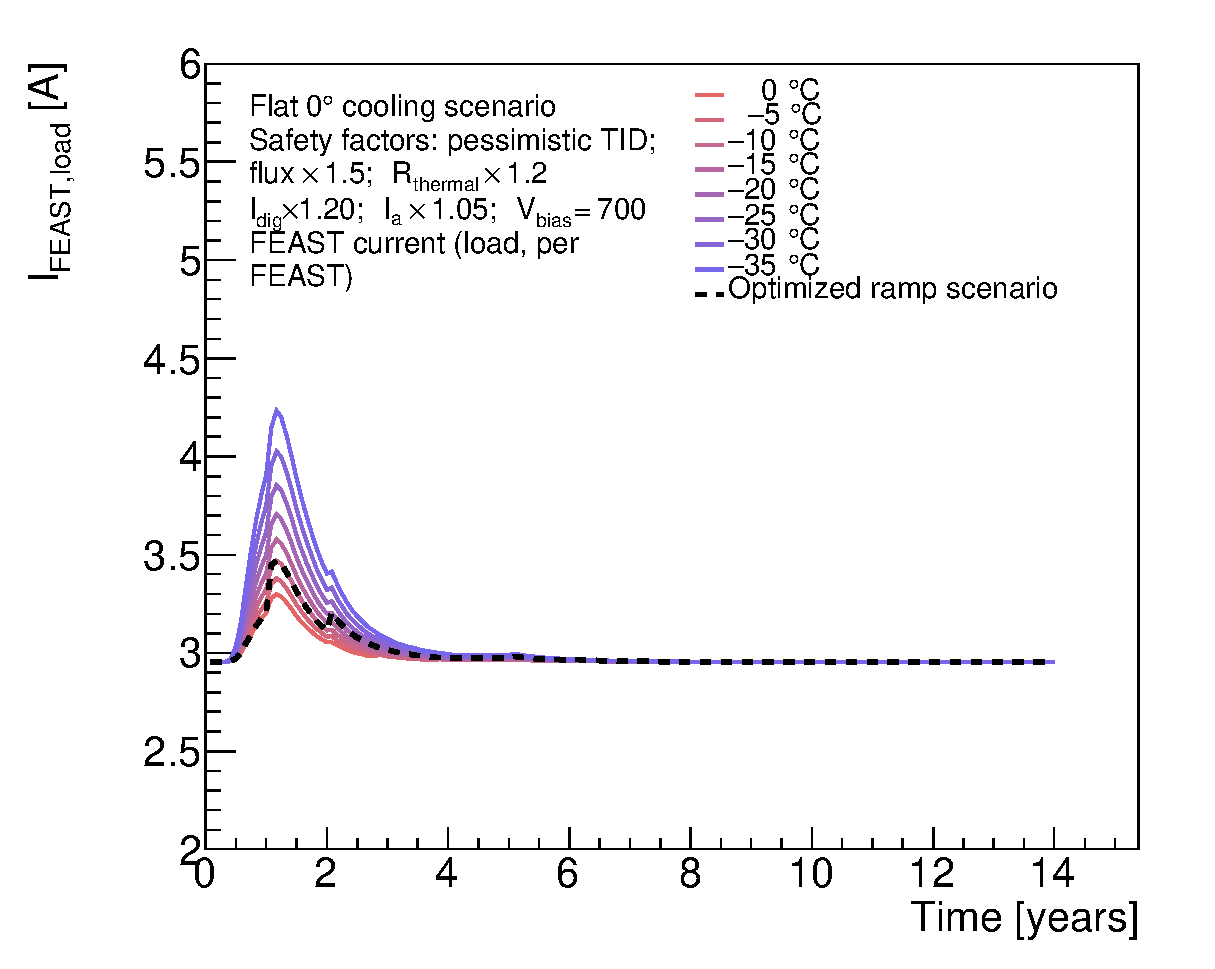
\includegraphics[width=0.45\linewidth]{figures/FeastCurrent_R1_newramp.eps}}
\caption{Performance of the cooling `ramp' scenario specified in Fig.~\ref{fig:coolant_ramp}. The dashed lines represents the ramp scenario, which has been selected so that the sensor leakage current (a) is stable throughout the lifetime of the ITk. A higher coolant temperature in the first few years reduces the TID effect, keeping the current load on the FEAST (b) well below its specified maximum of 4~A.}
\label{fig:rampoptimization}
\end{figure}
